	%% PART 6 : METHODES DE CONCEPTION	
	\newpage
	\subsection{Méthodes de conception}
		\subsubsection{Participative design : conception participative}
La conception participative est une méthode de travail utilisée principalement en conception de logiciel interactif. Sa principale caractéristique est la participation active des utilisateurs au travail de conception. Il s'agit donc d'une méthode de conception centrée sur l'utilisateur où l'accent est mis sur le rôle actif des utilisateurs \cite{wiki:cp}.

\paragraph{}
Il existe dans la littérature de nombreuses variantes de la méthode et de nombreuses techniques utilisées pour impliquer efficacement les utilisateurs. On peut noter particulièrement~:
\begin{itemize}
    \item l'observation et entretiens
    \item la production de scénarios
    \item le brainstorming
    \item le prototypage papier
    \item le prototypage vidéo
\end{itemize}

\paragraph{}
Une première séance de conception a lieu en début de projet : celle-ci regroupe les chercheurs et les développeurs de l'application, mais aussi les utilisateurs futurs ou potentiels. Intégrer les utilisateurs au processus de conception permet d'entrevoir au mieux leurs besoins et d'éviter un maximum d'erreurs d'interprétation ou d'oublis (voir illustration figure \ref{projet_info}). Les utilisateurs aident aussi à définir les problèmes éventuels et leurs possibles solutions.
\begin{figure}
	\centering
	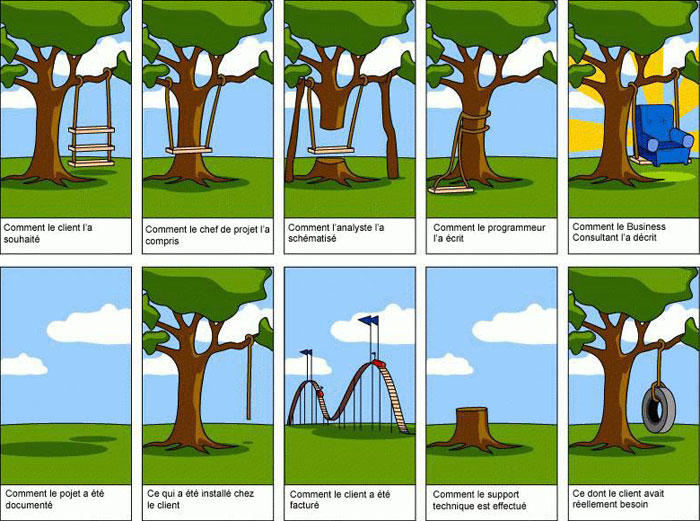
\includegraphics[width=16cm]{images/projet_info.jpg}
	\caption{Allégorie d'un projet informatique}
	\label{projet_info}
\end{figure}

\paragraph{}Par ailleurs, plusieurs séances peuvent avoir lieues tout au long du projet, afin de vérifier si les besoins ont évolués et si le développement actuel est effectivement en accord avec ceux-ci. Les utilisateurs aideront aussi l'équipe de recherche et développement à juger de la pertinence des solutions apportées.
\paragraph{}
D'un point de vue du développement, on notera que ce type de conception s'accorde parfaitement avec une méthodologie AGILE, et notamment la méthode SCRUM qui consiste en de courtes périodes de développement entre lesquelles on met en relief l'avancement par rapport au projet global.

		\subsubsection{Innovation games}
	Product Vision on : \\	
	http://www.joelonsoftware.com/articles/jimhighsmithonproductvisi.html \\
	Vaut le coup de faire un résumé?	
		\subsubsection{Impact mapping}
L'impact mapping est une technique de planification stratégique qui permet aux entreprises de ne pas s'égarer durant les phases de développement ou de livraison de projets, en identifiant clairement les hypothèses et en se concentrant sur l'impact que doit avoir le livrable, à la base du projet.

\paragraph{}
Les logiciels et projets fonctionnent en relation avec leur environnement. Ce sont des relations dynamiques et interdépendantes avec leurs utilisateurs, d'autres projets, l'entreprise et plus largement avec tout un écosystème. Pourtant, les méthodes actuelles de planification reposent soit sur le fait que cet environnement reste inchangé, soit ne permettent pas de donner une vision de haut niveau. L'impact mapping permet de visualiser la relation dynamique entre les livrables et leur environnement, capturant les hypothèses les plus importantes en même temps que le périmètre à livrer\cite{Adzi12}.		

\paragraph{}L'impact mapping contribue à réduire le gaspillage en évitant de trop élargir le périmètre fonctionnel ou de complexifier inutilement les solutions techniques à appporter. Cette technique permet de se concentrer sur les livrables en les mettant dans le contexte d'impact qu'ils sont censés avoir sur leur environnement. Elle améliore la collaboration en créant une vue haut-niveau que les responsables métier et les équipes de développement peuvent utiliser pour une meilleur priorisation, et comme une référence pour une mesure des progrès réalisés ayant vraiment un intérêt. Enfin, elle permet de s'assurer que les vrais objectifs métier sont atteints (ou que des projets peu réalistes sont stoppés avant qu'ils ne coûtent trop cher) en communiquant clairement les hypothèses qui ont justifiées ces projets, et en permettant tout au moins de les tester.

\paragraph{}L'impact mapping possède de nombreux avantages~:
	\begin{itemize}
	    \item Elle facilite la participation de groupes de personnes venant de métiers différents, aidant ainsi à tirer parti de la sagesse des foules.
	    \item Elle permet de visualiser des hypothèses. L'impact mapping permet aux équipes de prendre de meilleurs décisions dans un environnement changeant constamment comme les nouvelles technologies. La nature visuelle de cette méthode permet de tenir des réunions efficaces et renforce les réflexions haut-niveau, ce qui permet d'aligner les parties prenantes du projet.
	    \item C'est une méthode rapide. Pour cette raison, cette méthode s'insère parfaitement dans un processus de livraisons itératif qui devient courant de nos jours dans le domaine du logiciel.
	\end{itemize}
	
	\paragraph{\emph{Carte d'impact}\\}
Une carte d'impact est une visualisation du périmètre et des hypothèses sous-jacentes, créées de façon collaborative par des personnes senior, techniques et métier.
C'est une mind map développée durant une discussion et facilitée par le fait de répondre aux questions suivantes :
		\begin{itemize}
			\item \emph{Pourquoi ?} C'est la question la plus importante : Pourquoi faisons-nous ce que nous faisons? C'est l'objectif que nous voulons atteindre.
			\item \emph{Qui?}
Qui peut provoquer le changement attendu ? Qui peut l'empêcher ? Qui sont les clients ou utilisateurs de notre produit ? Qui sera impacté par celui-ci? Ce sont les acteurs qui peuvent influencer les résultats escomptés.
			\item \emph{Comment?}Comment le comportent des acteurs doit-il changer? Comment peuvent-ils nous aider à atteindre notre objectif? Comment peuvent-ils empêcher l'objectif de se réaliser? Ce sont les impacts que nous voulons créer.
			\item \emph{Quoi?}Que pouvons-nous faire, en tant qu'entreprise ou équipe de livraison, pour encourager ses impacts ? Ce sont les livrables, les caractéristiques du logiciel ou les activités de l'entreprise.
	\end{itemize}
\begin{figure}[htbp]
	\centering
	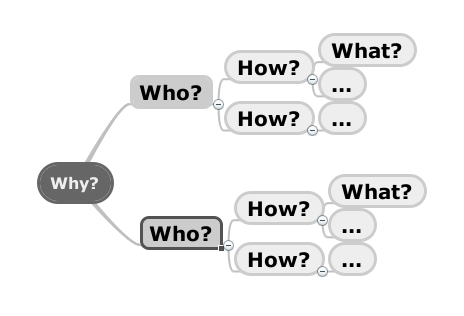
\includegraphics[scale=0.6]{images/impact_map.png}
	\caption{Carte d'impact}
	\label{impact_map}
\end{figure}